% Relatório: Análise de Eficácia de Testes com Teste de Mutação
% Compilar com pdfLaTeX + BibTeX (padrão do Overleaf).
\documentclass[12pt,oneside,a4paper,article,english,brazil]{abntex2}

\usepackage[T1]{fontenc}
\usepackage[utf8]{inputenc}
\usepackage{lmodern}
\usepackage{indentfirst}
\usepackage{graphicx}
\usepackage{float}
\usepackage{booktabs}
\usepackage{xcolor}
\usepackage{listings}
\usepackage[alf]{abntex2cite}

% ---------------------------------------------------------------------------
% DADOS DA CAPA — troque pelos seus dados
% ---------------------------------------------------------------------------
\newcommand{\disciplina}{Teste de Software}
\newcommand{\nomealuno}{SEU NOME COMPLETO}
\newcommand{\matricula}{SUA MATRÍCULA}

\titulo{Análise de Eficácia de Testes com Teste de Mutação}
\autor{\nomealuno}
\local{Belo Horizonte}
\data{2026}
\instituicao{Pontifícia Universidade Católica de Minas Gerais -- PUC Minas}

% ---------------------------------------------------------------------------
% Código-fonte
% ---------------------------------------------------------------------------
\definecolor{cinzafundo}{rgb}{0.96,0.96,0.96}
\definecolor{verdecom}{rgb}{0.20,0.45,0.20}
\definecolor{azulkw}{rgb}{0.10,0.20,0.60}
\lstset{
  language=Java, % sintaxe próxima de JavaScript
  morekeywords={function,const,let,expect,test,toBe,toThrow},
  basicstyle=\ttfamily\footnotesize,
  keywordstyle=\color{azulkw}\bfseries,
  commentstyle=\color{verdecom}\itshape,
  stringstyle=\color{red!60!black},
  backgroundcolor=\color{cinzafundo},
  frame=single, rulecolor=\color{gray!50},
  breaklines=true, columns=fullflexible, keepspaces=true,
  showstringspaces=false, aboveskip=6pt, belowskip=6pt,
  extendedchars=true,
  literate={á}{{\'a}}1 {à}{{\`a}}1 {ã}{{\~a}}1 {â}{{\^a}}1
           {é}{{\'e}}1 {ê}{{\^e}}1 {í}{{\'i}}1 {ó}{{\'o}}1
           {ô}{{\^o}}1 {õ}{{\~o}}1 {ú}{{\'u}}1 {ç}{{\c{c}}}1
           {Á}{{\'A}}1 {É}{{\'E}}1 {Í}{{\'I}}1 {Ó}{{\'O}}1
           {Ú}{{\'U}}1 {Ç}{{\c{C}}}1 {Ã}{{\~A}}1 {°}{{$^\circ$}}1
}
\renewcommand{\lstlistingname}{Código}

\hypersetup{colorlinks=true, linkcolor=black, citecolor=black, urlcolor=blue!50!black}
\setlength{\parindent}{1.25cm}
\setlength{\parskip}{0cm}
\setlength{\emergencystretch}{3em}

\begin{document}
\selectlanguage{brazil}
\frenchspacing

% ---------------------------------------------------------------------------
% CAPA
% ---------------------------------------------------------------------------
\begin{capa}
  \center
  {\ABNTEXchapterfont\large PONTIFÍCIA UNIVERSIDADE CATÓLICA DE MINAS GERAIS}

  \vspace{0.5cm}
  {\large \disciplina}

  \vfill
  {\ABNTEXchapterfont\large \nomealuno}

  \vspace{0.3cm}
  {\large Matrícula: \matricula}

  \vfill
  {\ABNTEXchapterfont\bfseries\LARGE \imprimirtitulo}

  \vfill
  \large PUC Minas

  \large \imprimirlocal

  \large \imprimirdata

  \vspace*{1cm}
\end{capa}

\textual

% ===========================================================================
\section{Introdução}
% ===========================================================================

Teste de mutação avalia a qualidade de uma suíte de testes inserindo pequenos
defeitos artificiais (\emph{mutantes}) no código -- por exemplo, trocar
\texttt{<} por \texttt{<=} ou \texttt{+} por \texttt{-} -- e executando os
testes contra cada versão alterada. Se algum teste falha, o mutante é
\emph{morto}; se todos passam, ele \emph{sobrevive}, o que indica que a suíte
não detectaria aquele defeito. A proporção de mutantes detectados é o
\emph{mutation score}.

O objetivo deste trabalho foi usar o StrykerJS \cite{stryker-docs} para medir a
eficácia da suíte Jest do projeto \texttt{operacoes-mutante}
\cite{tavares-repo}, uma biblioteca de 50 funções matemáticas em
\texttt{src/operacoes.js}, e fortalecê-la até um mutation score acima de 98\%,
sem alterar o código de produção.

% ===========================================================================
\section{Análise Inicial}
% ===========================================================================

A suíte original tem 50 testes, todos passando. A Tabela~\ref{tab:inicial}
mostra a cobertura obtida com \texttt{npm test -- --coverage} e o resultado da
primeira execução do Stryker (\texttt{coverageAnalysis: perTest}), que gerou
213 mutantes.

\begin{table}[htbp]
  \centering
  \caption{Cobertura de código e mutation score da suíte original}
  \label{tab:inicial}
  \begin{tabular}{lr@{\hspace{1.5cm}}lr}
    \toprule
    \multicolumn{2}{c}{Cobertura (Jest)} & \multicolumn{2}{c}{Mutação (Stryker)} \\
    \midrule
    Linhas     & 98,64\% & \textbf{Mutation score} & \textbf{73,71\%} \\
    Statements & 85,41\% & Killed + timeout        & 154 + 3 \\
    Branches   & 58,82\% & Survived                & 44 \\
    Funções    & 100\%   & No coverage             & 12 \\
    \bottomrule
  \end{tabular}
  \fonte{Elaborado pelo autor (2026).}
\end{table}

A diferença entre 98,64\% de linhas cobertas e 73,71\% de mutantes detectados
mostra o que cada métrica mede. Cobertura informa apenas que uma linha
\emph{foi executada} durante os testes; ela não verifica se alguma asserção
confere o resultado. O teste de mutação mede se as asserções \emph{percebem uma
mudança de comportamento}. Dos 56 mutantes não detectados, 44 estavam em
linhas cobertas. Os padrões mais comuns foram: só testar o caminho feliz de funções booleanas (\texttt{isPar},
\texttt{isEqual}, \texttt{isPrimo}), nunca testar as fronteiras das condições
(\texttt{n = 0}, \texttt{a = b}), usar \texttt{toThrow()} sem mensagem e usar
entradas que neutralizam a operação (como zero em multiplicações).

% ===========================================================================
\section{Análise de Mutantes Críticos}
% ===========================================================================

Três sobreviventes de mutadores diferentes \cite{stryker-mutators}, cada um
ilustrando uma fraqueza distinta da suíte:

\subsection{Mutante \#17: EqualityOperator em \texttt{raizQuadrada}}

\begin{figure}[H]
  \centering
  \caption{Mutante \#17 (linha 13) no relatório inicial do Stryker}
  \label{fig:m17}
  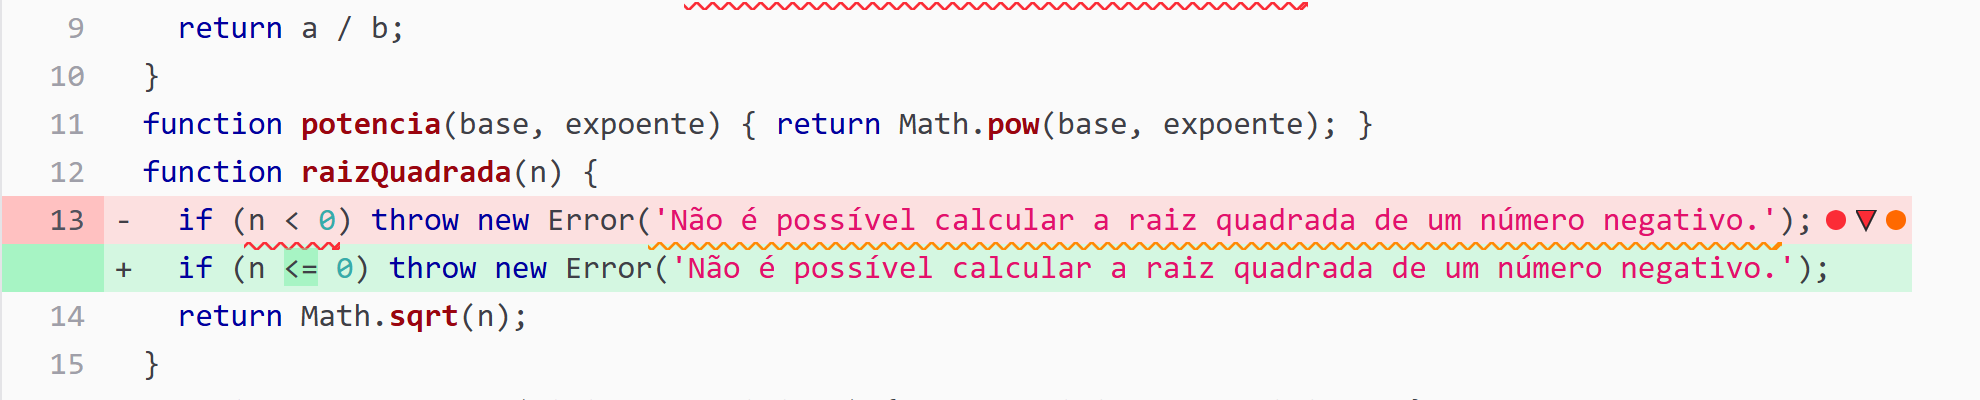
\includegraphics[width=0.66\textwidth]{figuras/recorte-17-raiz.png}
  \fonte{Relatório HTML do StrykerJS (2026).}
\end{figure}

\begin{lstlisting}
// original                      // mutado
if (n < 0) throw new Error(...);  if (n <= 0) throw new Error(...);
\end{lstlisting}

O Stryker transformou \texttt{<} em \texttt{<=} na guarda que rejeita números
negativos (Figura~\ref{fig:m17}). O único teste da função usa
\texttt{raizQuadrada(16)}, valor distante da fronteira: para qualquer
\texttt{n > 0} as duas versões se comportam igual. A diferença só aparece em
\texttt{n = 0}, que deveria retornar 0 e, no mutante, lança erro. É o caso
típico de \textbf{fronteira não testada}; como nenhum teste usava número
negativo, até o mutante que remove a condição (\#16) sobreviveu.

\subsection{Mutante \#160: ArithmeticOperator em \texttt{celsiusParaFahrenheit}}

\begin{figure}[H]
  \centering
  \caption{Mutante \#160 (linha 93) no relatório inicial do Stryker}
  \label{fig:m160}
  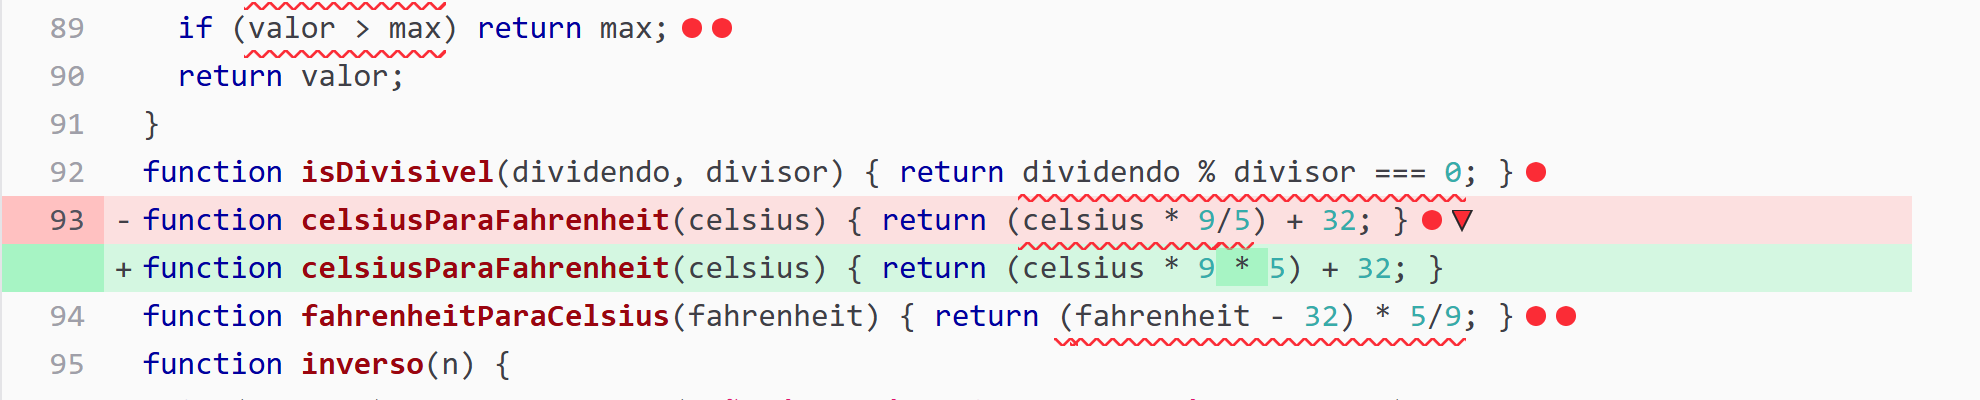
\includegraphics[width=0.66\textwidth]{figuras/recorte-160-celsius.png}
  \fonte{Relatório HTML do StrykerJS (2026).}
\end{figure}

\begin{lstlisting}
return (celsius * 9/5) + 32;   // original
return (celsius * 9 * 5) + 32; // mutado
\end{lstlisting}

O mutante troca a divisão por 5 por uma multiplicação (Figura~\ref{fig:m160}).
O teste original usa \texttt{celsius = 0}, e zero anula qualquer fator:
\texttt{0 * 9/5} e \texttt{0 * 9 * 5} valem 0, então as duas versões retornam
32. A \textbf{entrada escolhida mascara a mutação}: o teste só verifica a
parcela \texttt{+ 32}. O mesmo ocorreu em \texttt{fahrenheitParaCelsius(32)},
onde \texttt{32 - 32 = 0} esconde os mutantes \#163 e \#164.

\subsection{Mutante \#191: ConditionalExpression em \texttt{isEqual}}

\begin{figure}[H]
  \centering
  \caption{Mutante \#191 (linha 106) no relatório inicial do Stryker}
  \label{fig:m191}
  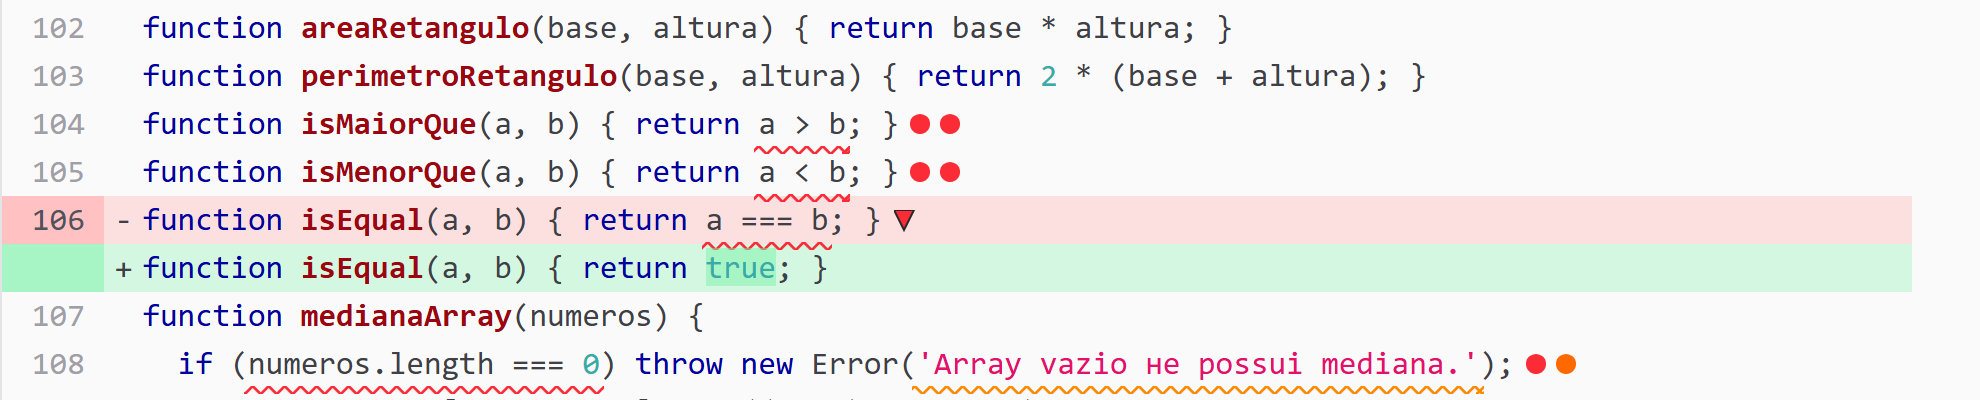
\includegraphics[width=0.66\textwidth]{figuras/recorte-191-isequal.png}
  \fonte{Relatório HTML do StrykerJS (2026).}
\end{figure}

\begin{lstlisting}
function isEqual(a, b) { return a === b; } // original
function isEqual(a, b) { return true; }    // mutado
\end{lstlisting}

O mutante substitui a comparação pela constante \texttt{true}
(Figura~\ref{fig:m191}). O único teste é \texttt{isEqual(7, 7)}, que espera
\texttt{true} -- exatamente o que uma função que sempre retorna \texttt{true}
entrega. A suíte tem uma \textbf{asserção unilateral}: verifica só o caso
positivo e nunca o negativo. O mesmo padrão explica os sobreviventes de
\texttt{isPar}, \texttt{isImpar}, \texttt{isDivisivel}, \texttt{isMaiorQue} e
\texttt{isMenorQue}.

% ===========================================================================
\section{Solução Implementada}
% ===========================================================================

Foram adicionados 29 testes em \texttt{test/operacoes.test.js}, cada um com
um comentário indicando o mutante que mata (id, posição e mutador). O
Código~\ref{cod:testes} mostra os que matam os três mutantes analisados.

\begin{lstlisting}[caption={Testes que matam os mutantes \#17, \#160 e \#191},label={cod:testes}]
test('raiz quadrada de zero é zero (fronteira de n < 0)', () => {
  // mata #17 (13:7 EqualityOperator): n < 0 -> n <= 0
  expect(raizQuadrada(0)).toBe(0);
});
test('converte 100 °C para 212 °F (entrada diferente de zero)', () => {
  // mata #160 (9/5 -> 9*5: daria 932) e #161 (celsius/9)
  expect(celsiusParaFahrenheit(100)).toBe(212);
});
test('isEqual retorna false para valores diferentes', () => {
  // mata #191 (106:33 ConditionalExpression -> true)
  expect(isEqual(7, 8)).toBe(false);
});
\end{lstlisting}

Os testes são eficazes porque cada um usa uma entrada em que o original e o
mutante produzem \emph{resultados diferentes}, e a asserção compara o valor
exato. \textbf{Fronteira}: \texttt{raizQuadrada(0)} fica no ponto em que
\texttt{<} e \texttt{<=} divergem (idem para \texttt{fatorial(0)},
\texttt{isPrimo(1)} e \texttt{isMaiorQue(5, 5)}). \textbf{Entrada não neutra}:
com \texttt{celsius = 100} cada operador gera um valor distinto (212 no
original, 932 com \texttt{9*5}, 34,2 com \texttt{/9}). \textbf{Caso negativo}:
\texttt{isEqual(7, 8)} exige \texttt{false}, o que nenhuma função constante
satisfaz junto com o teste positivo existente. Além disso,
\texttt{toThrow('mensagem')} matou tanto a remoção das guardas quanto a troca
das mensagens por string vazia, e arrays desordenados (\texttt{[5, 1, 3]},
\texttt{[4, 1, 3, 2]}) mataram os mutantes que removem ou alteram o
\texttt{sort} da mediana.

% ===========================================================================
\section{Resultados Finais}
% ===========================================================================

A Tabela~\ref{tab:final} mostra o mutation score subindo de 73,71\% para
98,12\% (209 de 213 mutantes detectados).

\begin{table}[htbp]
  \centering
  \caption{Comparação antes e depois da melhoria da suíte}
  \label{tab:final}
  \begin{tabular}{lrr}
    \toprule
    Métrica & Antes & Depois \\
    \midrule
    Número de testes          & 50      & 79 \\
    Cobertura de linhas       & 98,64\% & 100\% \\
    Cobertura de branches     & 58,82\% & 100\% \\
    \textbf{Mutation score}   & \textbf{73,71\%} & \textbf{98,12\%} \\
    Killed                    & 154     & 206 \\
    Timeout                   & 3       & 3 \\
    Survived                  & 44      & 4 \\
    No coverage               & 12      & 0 \\
    \bottomrule
  \end{tabular}
  \fonte{Elaborado pelo autor (2026).}
\end{table}

% Visão geral do relatório final (opcional, ocupa espaço):
% \begin{figure}[htbp]
%   \centering
%   \caption{Visão geral do relatório final do Stryker}
%   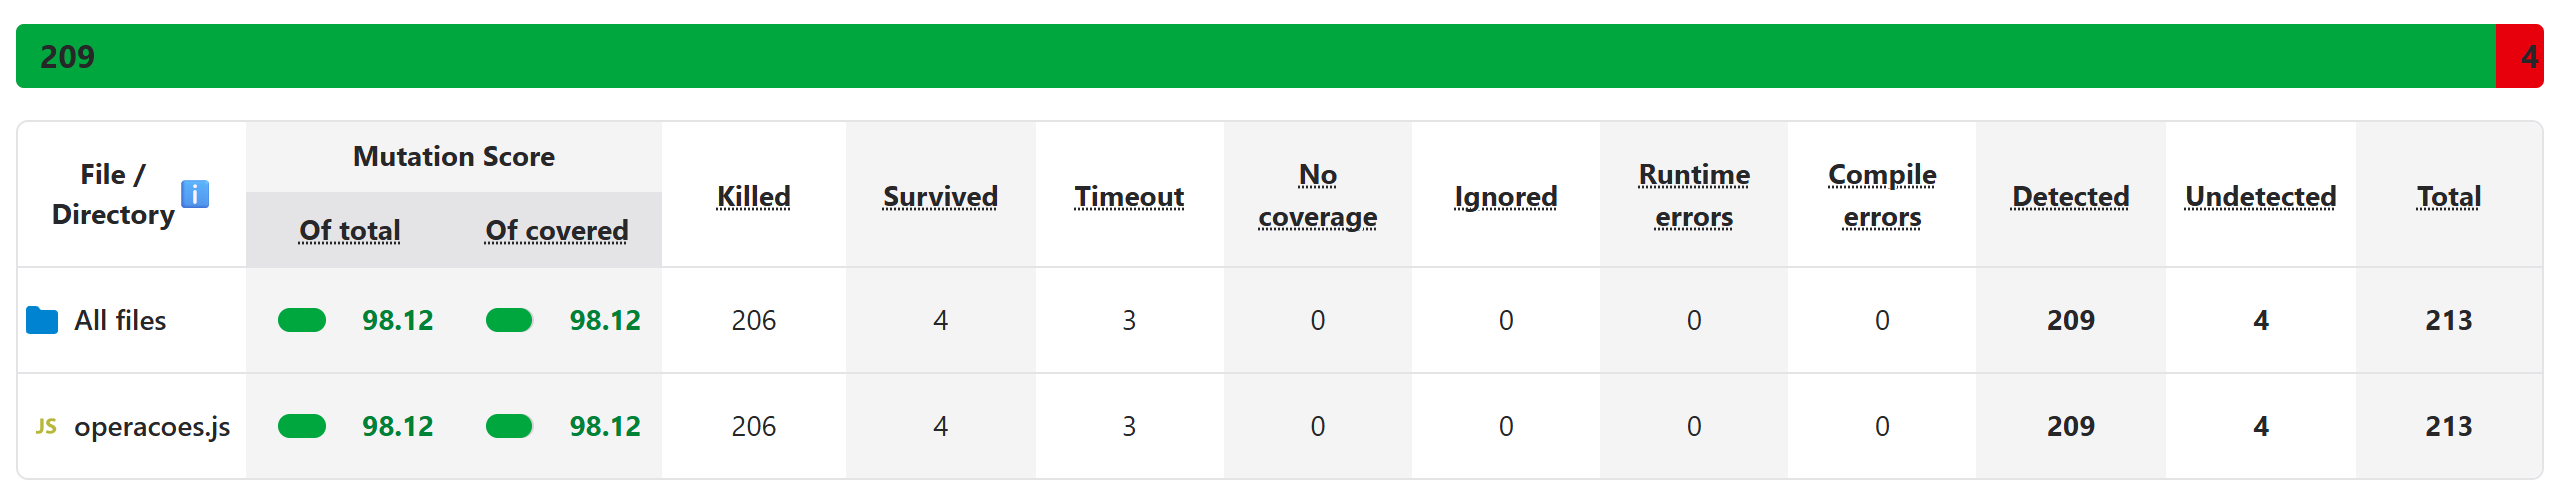
\includegraphics[width=0.8\textwidth]{figuras/visao-geral-final.png}
%   \fonte{Relatório HTML do StrykerJS (2026).}
% \end{figure}

\textbf{Mutantes equivalentes restantes.} Os 4 sobreviventes (\#31, \#32, \#33,
\#35) removem ou enfraquecem a guarda \texttt{if (n === 0 || n === 1) return 1;}
de \texttt{fatorial}. São equivalentes: sem ela, para \texttt{n} igual a 0 ou 1
o laço \texttt{for (let i = 2; i <= n; i++)} não itera e a função retorna o
mesmo valor 1, então nenhum teste pode matá-los.

\textbf{Casos de borda.} Três mutantes só morreram com entradas incomuns:
em \texttt{clamp}, \texttt{<}$\to$\texttt{<=} (\#147) e \texttt{>}$\to$\texttt{>=}
(\#151) só se distinguem com zero com sinal (\texttt{clamp(-0, 0, 10)} devolve
\texttt{-0} no original e \texttt{0} no mutante; \texttt{toBe} usa
\texttt{Object.is}), e a guarda de \texttt{produtoArray} (\#140) só importa para
um array-like vazio sem \texttt{reduce}. Sem eles, o score seria 96,71\%.

% ===========================================================================
\section{Conclusão}
% ===========================================================================

A suíte original tinha 98,64\% de cobertura de linhas e, mesmo assim, deixava
passar mais de um quarto dos defeitos simulados: a cobertura mostrava só que o
código era executado, não que as asserções eram fortes. O teste de mutação
expôs cada fraqueza com linha e alteração exatas. O score exige interpretação,
pois há mutantes equivalentes, mas usado com análise ele complementa a
cobertura: esta mostra o que nunca foi exercitado; a mutação, o que foi
exercitado sem ser verificado.

% ---------------------------------------------------------------------------
\postextual
\bibliography{referencias}

\end{document}
